\documentclass{article}

% if you need to pass options to natbib, use, e.g.:
% \PassOptionsToPackage{numbers, compress}{natbib}
% before loading nips_2016
%
% to avoid loading the natbib package, add option nonatbib:
% \usepackage[nonatbib]{nips_2016}

%\usepackage{nips_2016}

% to compile a camera-ready version, add the [final] option, e.g.:
\usepackage[final]{nips_2016}

\usepackage[utf8]{inputenc} % allow utf-8 input
\usepackage[T1]{fontenc}    % use 8-bit T1 fonts
\usepackage{hyperref}       % hyperlinks
\usepackage{url}            % simple URL typesetting
\usepackage{booktabs}       % professional-quality tables
\usepackage{amsfonts}       % blackboard math symbols
\usepackage{nicefrac}       % compact symbols for 1/2, etc.
\usepackage{microtype}      % microtypography
\usepackage{color}
\usepackage{graphicx}
\usepackage{amssymb,amsfonts,amsmath,graphicx}      
\graphicspath{ {../figures/} }

\newcommand{\ind}[1]{1_{#1}} % Indicator function
\newcommand{\pr}{P} % Generic probability
\newcommand{\ex}{E} % Generic expectation
\newcommand{\var}{\textrm{Var}}
\newcommand{\cov}{\textrm{Cov}}
\newcommand{\sgn}{\textrm{sgn}}
\newcommand{\sign}{\textrm{sign}}
\newcommand{\kl}{\textrm{KL}} 
\newcommand{\abs}[1]{|{#1}|}



\renewcommand{\S}{\Sigma}
\renewcommand{\L}{\Lambda}
\renewcommand{\[}{\begin{equation}}
\renewcommand{\]}{\end{equation}}
\renewcommand{\b}{\backslash}
\newcommand{\g}{\,\vert\,}
\newcommand{\tr}{\mathrm{tr}}
\newcommand{\diag}{\mathrm{diag}}
\newcommand{\bea}{\begin{eqnarray}}
\newcommand{\eea}{\end{eqnarray}}
\newcommand{\hx}{\hat{x}}
\newcommand{\hxi}{\hat{\xi}}
\newcommand{\Var}{\mathrm{Var}}
\newcommand{\Cov}{\mathrm{Cov}}
\newcommand{\prop}{\propto}
\newcommand{\deq}{:=}

\newcommand{\EE}{\mathbb{E}}
\newcommand{\II}{\mathbb{I}}
\newcommand{\R}{\mathbb{R}}
\newcommand{\PP}{\mathbb{P}}

\newcommand{\La}{\mathcal{L}}

\newcommand{\n}{\mathcal{N}}

\newcommand{\bx}{\mathbf{x}}
\newcommand{\bX}{\mathbf{X}}
\newcommand{\by}{\mathbf{y}}
\newcommand{\bs}{\mathbf{s}}
\newcommand{\bn}{\mathbf{n}}
\newcommand{\br}{\mathbf{r}}
\newcommand{\bt}{\mathbf{t}}

\newcommand{\fig}[1]{Figure~\ref{fig:#1}}
\newcommand{\chap}[1]{Chapter~\ref{chap:#1}}
\newcommand{\mysec}[1]{Section~\ref{sec:#1}}
\newcommand{\app}[1]{Appendix~\ref{sec:#1}}
\newcommand{\eq}[1]{Eq.~(\ref{eq:#1})}
\newcommand{\eqs}[1]{Eqs.~(\ref{eq:#1})}
\newcommand{\eqss}[1]{(\ref{eq:#1})}
\newcommand{\thm}[1]{Theorem~\ref{thm:#1}}

\newcommand{\indep}{{\;\bot\!\!\!\!\!\!\bot\;}}
\newcommand{\eps}{\varepsilon}

\newcommand{\one}{1}
\newcommand{\Dir}{{\rm Dir}}
\newcommand{\Mult}{{\rm Mult}}
\newcommand{\Bin}{{\rm Bin}}
\newcommand{\Ga}{{\rm Ga}}
\newcommand{\IG}{{\rm IG}}
\newcommand{\InvGa}{{\rm IG}}
\newcommand{\Chisquare}{\Chi^2}
\newcommand{\St}{{\rm St}}
\newcommand{\Beta}{{\rm Beta}}
\newcommand{\iid}{i.i.d.}
\newcommand{\Eta}{{\cal N}}
\newcommand{\Ber}{{\rm Ber}}

\newcommand{\simiid}{\stackrel{\tiny\text{iid}}{\sim}}
\newcommand{\simind}{\stackrel{\tiny\text{ind}}{\sim}}

\DeclareMathOperator*{\BP}{BP}
\DeclareMathOperator*{\DP}{DP}
\DeclareMathOperator*{\GP}{GP}
\DeclareMathOperator*{\BeP}{BeP}

% Caligraphic alphabet
\newcommand{\calr}{\mathcal{R}} % only because \cr already taken
\newcommand{\ca}{\mathcal{A}} \newcommand{\cb}{\mathcal{B}} \newcommand{\cc}{\mathcal{C}} \newcommand{\cd}{\mathcal{D}} \newcommand{\ce}{\mathcal{E}} \newcommand{\cf}{\mathcal{F}} \newcommand{\cg}{\mathcal{G}} \newcommand{\ch}{\mathcal{H}} \newcommand{\ci}{\mathcal{I}} \newcommand{\cj}{\mathcal{J}} \newcommand{\ck}{\mathcal{K}} \newcommand{\cl}{\mathcal{L}} \newcommand{\cm}{\mathcal{M}} \newcommand{\cn}{\mathcal{N}} \newcommand{\co}{\mathcal{O}} \newcommand{\cp}{\mathcal{P}} \newcommand{\cq}{\mathcal{Q}} \newcommand{\cs}{\mathcal{S}} \newcommand{\ct}{\mathcal{T}} \newcommand{\cu}{\mathcal{U}} \newcommand{\cv}{\mathcal{V}} \newcommand{\cw}{\mathcal{W}} \newcommand{\cx}{\mathcal{X}} \newcommand{\cy}{\mathcal{Y}} \newcommand{\cz}{\mathcal{Z}}

% Convergence
\newcommand{\convd}{\stackrel{d}{\longrightarrow}} % convergence in distribution/law/measure
\newcommand{\convp}{\stackrel{P}{\longrightarrow}} % convergence in probability
\newcommand{\convas}{\stackrel{\textrm{a.s.}}{\longrightarrow}} % convergence almost surely
\newcommand{\convr}{\stackrel{r}{\longrightarrow}} % convergence in r^{th} mean

\newcommand{\eqd}{\stackrel{d}{=}} % equal in distribution/law/measure
\newcommand{\argmax}{\mathop{\mathrm{argmax}}}
\newcommand{\argmin}{\mathop{\mathrm{argmin}}}
\newcommand{\conv}{\textrm{conv}} % for denoting the convex hull


\makeatletter
\providecommand*{\diff}%
	{\@ifnextchar^{\DIfF}{\DIfF^{}}}
\def\DIfF^#1{%
	\mathop{\mathrm{\mathstrut d}}%
		\nolimits^{#1}\gobblespace}
\def\gobblespace{%
	\futurelet\diffarg\opspace}
\def\opspace{%
	\let\DiffSpace\!%
	\ifx\diffarg(%
		\let\DiffSpace\relax
	\else
		\ifx\diffarg[%
			\let\DiffSpace\relax
	\else
		\ifx\diffarg\{%
			\let\DiffSpace\relax
		\fi\fi\fi\DiffSpace}


\providecommand*{\deriv}[3][]{\frac{\diff^{#1}#2}{\diff #3^{#1}}}
\providecommand*{\pderiv}[3][]{\frac{\partial^{#1}#2}{\partial #3^{#1}}}
		
\newcommand{\threequals}{\equiv}

\usepackage{subcaption}

\title{Formatting instructions for NIPS 2016}

% The \author macro works with any number of authors. There are two
% commands used to separate the names and addresses of multiple
% authors: \And and \AND.
%
% Using \And between authors leaves it to LaTeX to determine where to
% break the lines. Using \AND forces a line break at that point. So,
% if LaTeX puts 3 of 4 authors names on the first line, and the last
% on the second line, try using \AND instead of \And before the third
% author name.

\author{
  Elijahu Ben-Michael \\
  Department of Statistics\\
  UC Berkeley
  %% examples of more authors
   \And
  Runjing Liu \\
  Department of Statistics\\
  UC Berkeley
  %% \texttt{email} \\
   \AND
  Jake Soloff \\
  Department of Statistics\\
  UC Berkeley
  %% \texttt{email} \\
  %% \And
  %% Coauthor \\
  %% Affiliation \\
  %% Address \\
  %% \texttt{email} \\
  %% \And
  %% Coauthor \\
  %% Affiliation \\
  %% Address \\
  %% \texttt{email} \\
}

\begin{document}
% \nipsfinalcopy is no longer used

\maketitle

\begin{abstract}
  The abstract paragraph should be indented \nicefrac{1}{2}~inch
  (3~picas) on both the left- and right-hand margins. Use 10~point
  type, with a vertical spacing (leading) of 11~points.  The word
  \textbf{Abstract} must be centered, bold, and in point size 12. Two
  line spaces precede the abstract. The abstract must be limited to
  one paragraph.
\end{abstract}

\section{Introduction}





\subsection{Motivation} 
Voting records of legislators are commonly used by political scientists to examine relationships between legislator policy preferences, institutional structures, and legislative outcomes (Clinton et al 2004). In fact, even simple dimensionality reduction techniques on roll call data are able to uncover the political characteristics of individual representatives. For example, in figure \ref{fig:NNMF}, we factored the $448\times1707$ matrix representing the 448 representatives and their votes on 1707 bills into two nonnegative matrices of dimensions $448\times 2$ and $2\times 1707$ . Plotting the  $448\times 2$ matrix where each row places a representative in a two dimensional space, we are able to clearly identify party affiliation. \par

Another dimensionality technique we applied to visualize voting data was principle component analysis (figure \ref{fig:PCA}). We formed the principle components by computing the two largest eigenvalues and their respective eigenvectors on the $448\times 448$ covariance matrix of vote data, and each representative's voting profile was projected onto the space spanned by these principle components. Again, we clearly see differentiation along party lines. 



\begin{figure}[h]
  \centering
    \begin{subfigure}[b]{0.4\textwidth}
        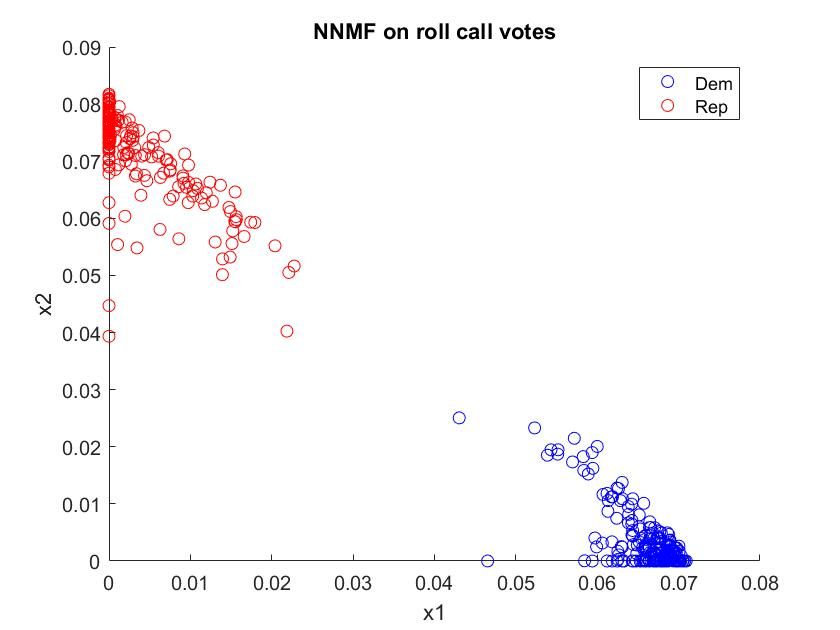
\includegraphics[width=\textwidth]{NNMF_votes.jpg}
        \caption{}
        \label{fig:NNMF}
    \end{subfigure}
          \begin{subfigure}[b]{0.4\textwidth}
        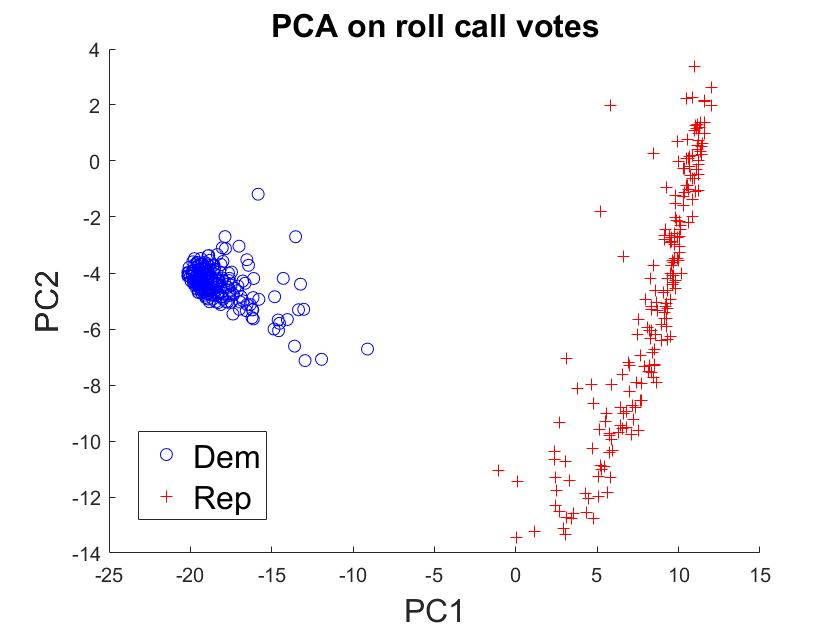
\includegraphics[width=\textwidth]{PCA_votes}
        \caption{}
        \label{fig:PCA}
    \end{subfigure}
  \caption{(a) Nonnegative matrix factorization on the $448\times 1707$ matrix (448 representatives, 1707 bills) of roll call votes into two matrices of dimensions $448\times 2$ and $2\times 1707$. The rows of the $448\times 2$ matrices were plotted to visualize the distribution of representatives. (b) Principle component analysis on the roll call vote data. The eigenvalues and eigenvectors of the $448\times 448$ covariance matrix of representative voting data were computed, and each representative's voting profile was projected onto the space of the two eigenvectors with the two largest eigenvalues.}
\end{figure}

Another common analysis of roll call votes that may potentially yield more subtle structures in legislative preferences is to conduct {\itshape ideal point modeling}. {\color{red} maybe the next sentences goes in the introduction \{} Here, a congressman and a bill is presumed to lie in a latent `'ideological space,'' where the probability of a ``yay'' or ``nay'' response is a function of the bill's position and the congressman's position. The congressman's position is known as an `'ideal point'' because his or her utility decreases as a bill's position deviates from this point. {\color{red} \}}

In Gerrish and Blei 2011, ideal points of each representative was drawn from a zero mean Gaussian prior. In this paper, we aim to obtain better estimates of the representatives' ideal points, and to do so, we incorporate data from caucus memberships using a stochastic block model (see models below) because we hypothesize that sharing caucuses with other representatives influences a representative's voting behavior. Figure \ref{fig:VotesVsCaucus} plots the number of shared caucuses between two representatives against the proportion of bills on which they voted the same way, and we see that the more caucuses two members share, the more likely they are to vote the same way. 

\begin{figure}[h]
  \centering
        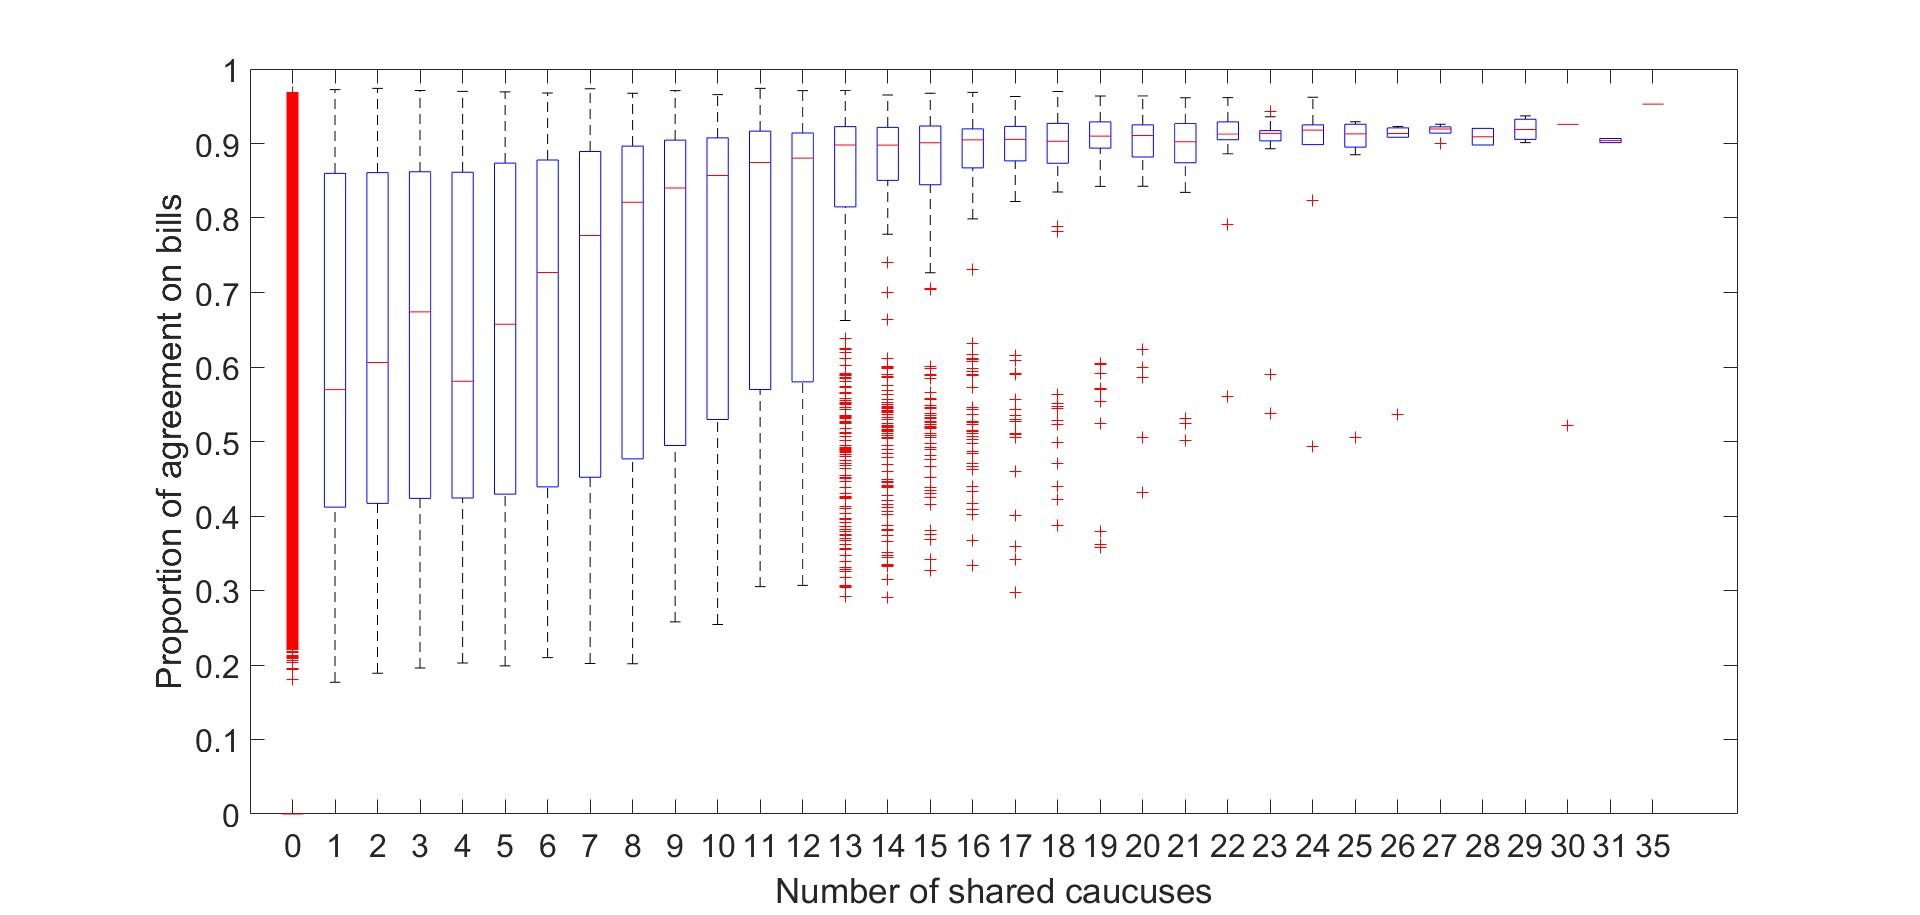
\includegraphics[width=\textwidth]{Caucus_vs_Votes.jpg}
  \caption{The distribution of agreement on bills as a function of the number of caucuses two representatives share. We see that the more caucuses people share, the more likely they are to agree on a bill. }
          \label{fig:VotesVsCaucus}
\end{figure}

Moreover, figure \ref{fig:Nhood_Caucus} shows the relationship between representatives within several caucuses in an undirected graphical model. We first used roll call vote data to infer the graph structure among the representatives in the entire House; we assumed pairwise interactions described via an Ising model in which each node denotes a binary variable of a representative voting either yes or no. The edges were inferred using neighborhood selection, and the graphs shown in figure \ref{fig:Nhood_Caucus} are subsets of this full graph corresponding to members of a caucus. The connectivity ( \#edges /\#nodes(\#nodes-1) ) of the full graph with 448 representatives is 0.064, while the connectivity within the caucus subgraphs was much higher. This suggests that a representative more likely to be influenced by a member of his caucus than another  random representative in the House. Therefore, by relating these interactions among representatives to their ideal points using a stochastic block model, we hope to be able to capture more subtle patterns in estimating ideal points. In particular, we aim to extend the one dimensional ideological space in Gerrish and Blei to higher dimensions. In doing so, we hypothesize that more accurate predictions of roll call votes can be explained. 


% The connection between caucus memberships and ideal points are described by a {\itshape stochastic block model} (see below). 

%This model posits that the representatives are grouped by latent communites, and these communities manifest themselves in a representative's ideal point (representatives in the same community are likely to have similar ideal points) and in a representative's caucus membership (representatives in the same community are likely to share many caucuses). 




\begin{figure}[h]
  \centering
    \begin{subfigure}[b]{0.49\textwidth}
        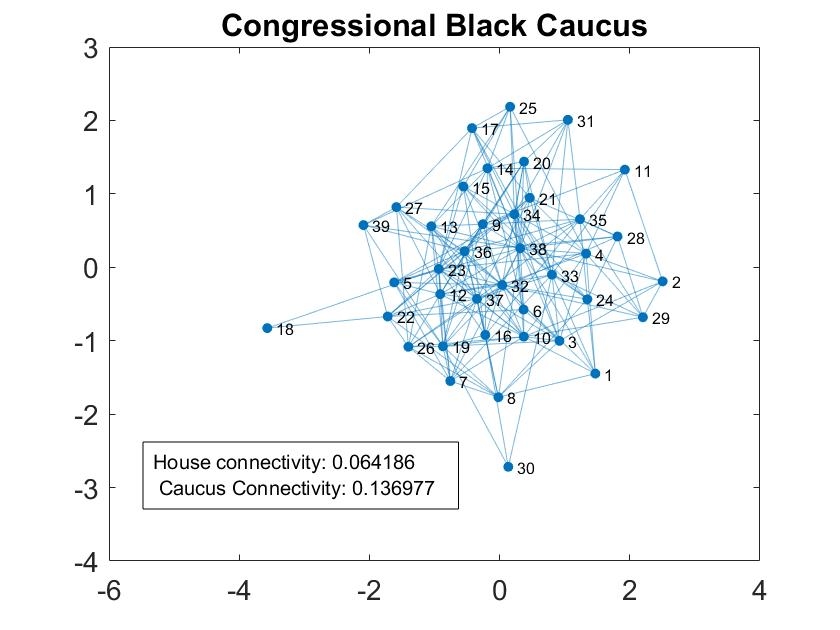
\includegraphics[width=\textwidth]{/Neighborhood_Regression/Congressional_Black_Caucus.jpg}
        \caption{}
    \end{subfigure}
          \begin{subfigure}[b]{0.49\textwidth}
        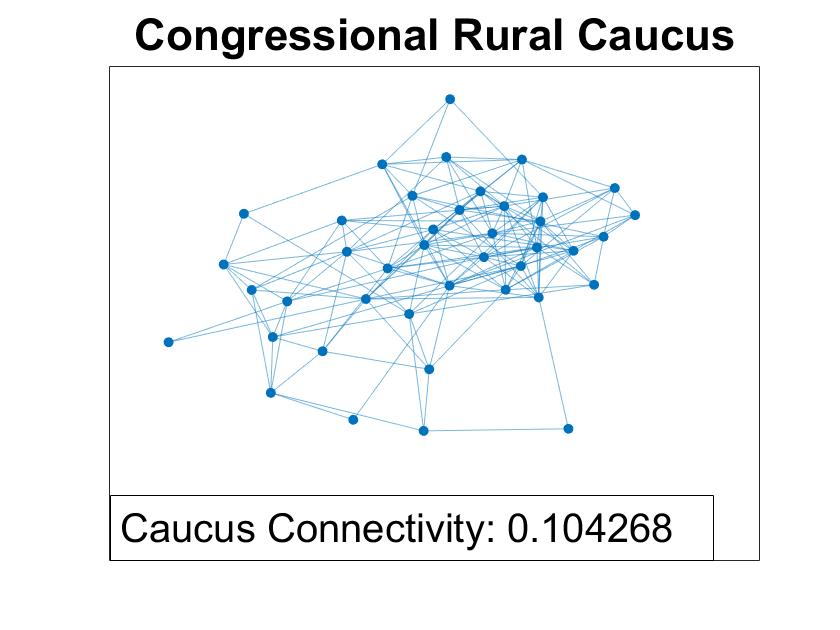
\includegraphics[width=\textwidth]{/Neighborhood_Regression/Congr_Rural_Caucus.jpg}
        \caption{}
    \end{subfigure}
        \begin{subfigure}[b]{0.49\textwidth}
        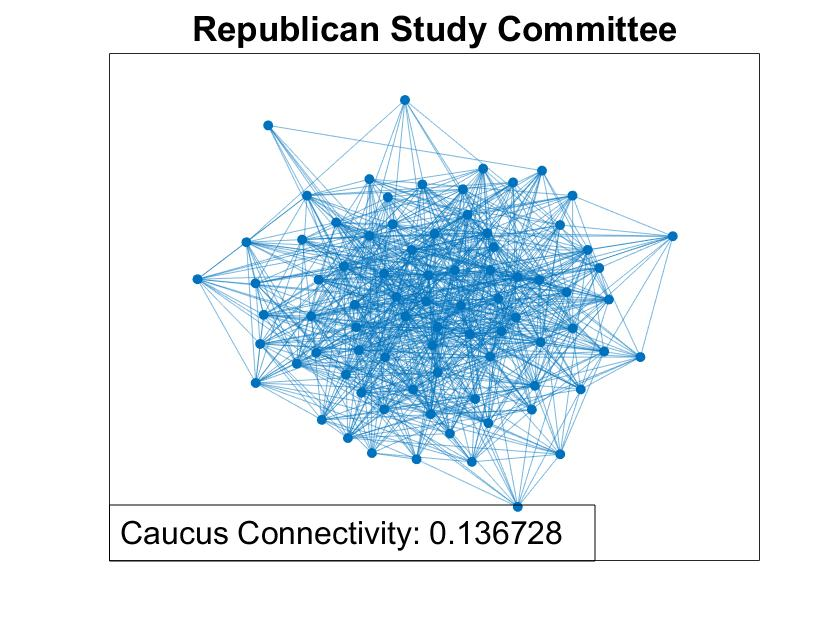
\includegraphics[width=\textwidth]{/Neighborhood_Regression/Rep_Study_Committee.jpg}
        \caption{}
    \end{subfigure}
          \begin{subfigure}[b]{0.49\textwidth}
        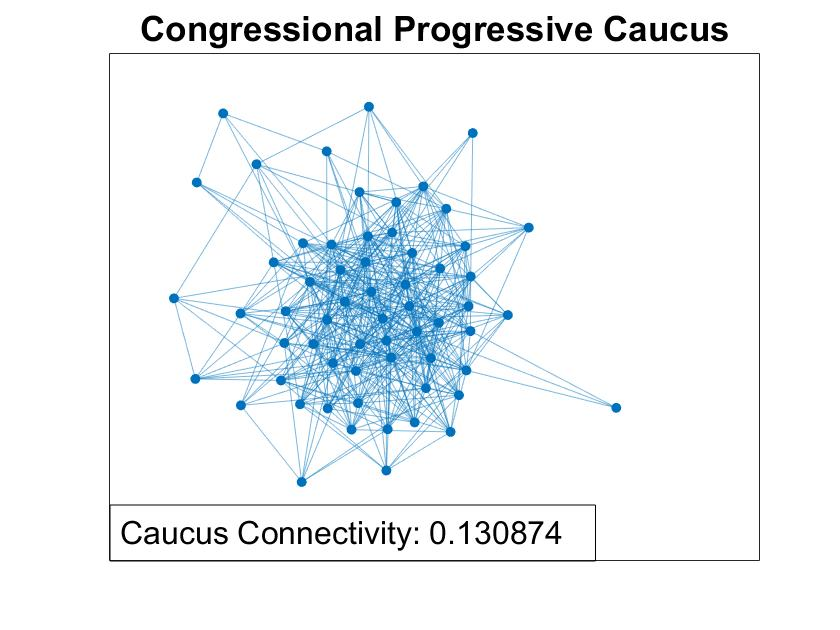
\includegraphics[width=\textwidth]{/Neighborhood_Regression/Congr_Prog_Caucus.jpg}
        \caption{}
    \end{subfigure}
  \caption{Graphs inferred from Neighborhood regression on House roll call vote data. Shown here are subgraphs with representatives taken from a given caucus. The caucuses are their connectivities shown here are (a) the Congressional Black Caucus, connectivity 0.137; (b) the Congressional Rural Caucus, connectivity 0.104; (c) the Republican Study Committee, connectivity 0.136; and (d) the Congressional Progressive Caucus, connectivity 0.131. In each case, the connectivity within the caucuses was higher than the connectivity of the whole graph of the House (0.064).}
      \label{fig:Nhood_Caucus}
\end{figure}




\section{The model}
We introduce models for both roll call votes and caucus memberships. 

\subsection{Ideal point model}

\subsection{Stochastic Block Model}


\section{Results}

\section{Discussion}




\section*{References}

\medskip

\small

[1] Gerrish, S.M.\ \& Blei, M.B. \ (2011) Predicting Legislative Roll Calls from Text. {\it Proceedings of the 28th International Conference on Machine Learning}

\appendix

\section{Variational updates}

\end{document}